\documentclass{article}
\usepackage{markdown}
\usepackage{soulutf8}
%\renewcommand{\st}[1]{}
%\usepackage[scale=.75]{geometry}
\usepackage{placeins}
\usepackage{amsthm,amssymb,hyperref,marginnote}
\usepackage{subfig}
\usepackage{enotez}
\setenotez{counter-format=Alph}
\usepackage[textsize=footnotesize]{luatodonotes}%\usepackage{todonotes}%
\usepackage{xcolor}
\newcommand{\nb}[1]{%
  \todo[color=blue!60!black,shadow]{NB:\\ #1}%
}

\usepackage{newunicodechar}
% misc
\newunicodechar{∆}{\ensuremath{\Delta}}
\newunicodechar{⦄}{\ensuremath{\}}}
\newunicodechar{⦃}{\ensuremath{\{}}
\newunicodechar{¯}{\ensuremath{{}^{-}}}
\newunicodechar{·}{\ensuremath{\cdot}}
\newunicodechar{·}{\ensuremath{\cdot}}
\newunicodechar{∫}{\ensuremath{\int}}
\newunicodechar{□}{\Box}
\newunicodechar{⊗}{\ensuremath{\otimes}}
\newunicodechar{★}{\ensuremath{\star}}
\newunicodechar{∗}{^*}
\newunicodechar{♯}{\sharp}
\newunicodechar{①}{(1)}
\newunicodechar{②}{(2)}
\newunicodechar{☺}{\ensuremath{\smiley}}
\newunicodechar{⊣}{\ensuremath{\dashv}}

% advanced typography stuff
\newunicodechar{“}{``}
\newunicodechar{”}{''}
% \newunicodechar{„}{\glqq}


\newunicodechar{fi}{fi}
\newunicodechar{ff}{ff}
\newunicodechar{fl}{fl}
% \newunicodechar{ü}{{\"{u}}}
% \newunicodechar{ä}{{\"{a}}}
% \newunicodechar{ö}{{\"{o}}}
\newunicodechar{∖}{\ensuremath{\setminus}}

%math symbols
\newunicodechar{∃}{\exists}
\newunicodechar{∀}{\ensuremath{\forall}}
\newunicodechar{⇒}{\ensuremath{\Rightarrow}}
\newunicodechar{⇔}{\Leftrightarrow}

% white spaces, etc
%\DeclareUnicodeCharacter{00A0}{~}%\newunicodechar{ }{~}
\newunicodechar{␣}{\_}
\newunicodechar{…}{\ifmmode\dotsc\else\ldots\fi}
\newunicodechar{⋯}{\dotsm}
\newunicodechar{–}{\textendash}


% SUBSCRIPTS
%% letters
\newunicodechar{ₙ}{_n}
\newunicodechar{ₘ}{_m}
\newunicodechar{ₕ}{_h}
\newunicodechar{ᵢ}{_i}
\newunicodechar{ⱼ}{_j}
\newunicodechar{ₖ}{_k}
\newunicodechar{ₜ}{_t}
\newunicodechar{ₛ}{_s}
\newunicodechar{ᵤ}{_u}
\newunicodechar{ᵥ}{_v}
%% numbers
\newunicodechar{₀}{\ensuremath{{}_0}}
\newunicodechar{₁}{\ensuremath{{}_1}}
\newunicodechar{₂}{_2}
\newunicodechar{₆}{_6}

% superscripts
\newunicodechar{ⁿ}{^n}
\newunicodechar{ᵐ}{^m}
\newunicodechar{ˢ}{^s}
\newunicodechar{ᵗ}{\ensuremath{{}^t}}
\newunicodechar{ⁱ}{^i}
\newunicodechar{ʲ}{^j}
\newunicodechar{ᵏ}{^k}
\newunicodechar{ᵗ}{^t}
\newunicodechar{¹}{\ensuremath{{}^1}}
\newunicodechar{²}{^2}
\newunicodechar{³}{^3}
\newunicodechar{ᵀ}{^{\rm T}}


% constants and scalarlike
\newunicodechar{∞}{\infty}

% math operators
%\DeclareUnicodeCharacter{00D7}{\ensuremath{\times}}%\newunicodechar{×}{\times}
\newunicodechar{÷}{\div}
%\DeclareUnicodeCharacter{2190}{\ensuremath\leftarrow}%\newunicodechar{←}{\ensuremath\leftarrow}
%\DeclareUnicodeCharacter{2192}{\ensuremath\rightarrow}%\newunicodechar{→}{\ensuremath\rightarrow}
%\DeclareUnicodeCharacter{21E2}{\ensuremath\dashrightarrow}%\newunicodechar{⇢}{\ensuremath\dashrightarrow}
%\DeclareUnicodeCharacter{21A6}{\ensuremath\mapsto}%\newunicodechar{↦}{\ensuremath\mapsto}
%\DeclareUnicodeCharacter{2196}{\ensuremath\nwarrow}%↖
%\DeclareUnicodeCharacter{2197}{\ensuremath\nearrow}%↗
%\DeclareUnicodeCharacter{2198}{\ensuremath\searrow}%↘
%\DeclareUnicodeCharacter{2199}{\ensuremath\swarrow}%↙
        
% sets 
\newunicodechar{∅}{\varnothing}

% analysis
\newunicodechar{∫}{\int}
\newunicodechar{ℓ}{\ell}

% math relation symbols
\newunicodechar{∈}{\ensuremath{\in}}
\newunicodechar{∉}{\notin}
\newunicodechar{∋}{\ni}
\newunicodechar{≅}{\cong}
\newunicodechar{≥}{\geq}
\newunicodechar{≤}{\leq}
\newunicodechar{≪}{\ll}
\newunicodechar{≫}{\rr}
\newunicodechar{⋘}{\lll}
\newunicodechar{⋙}{\rrr}
%\DeclareUnicodeCharacter{2260}{\neq}%\newunicodechar{≠}{\neq}
\newunicodechar{⊂}{\subset}
\newunicodechar{⊆}{\ensuremath{\subseteq}}
\newunicodechar{⊃}{\supset}
\newunicodechar{⊇}{\supseteq}
\newunicodechar{⊑}{\sqsubseteq}
\newunicodechar{⊒}{\sqsupseteq}

% binary operators
\newunicodechar{⋃}{\bigcup}
\newunicodechar{∪}{\ensuremath{\cup}}
\newunicodechar{⋂}{\bigcap}
\newunicodechar{∩}{\cap}
\newunicodechar{∘}{\circ}

% math arrows 
\newunicodechar{↑}{\ensuremath{\uparrow}}
\newunicodechar{↓}{\ensuremath{\downarrow}}

\newunicodechar{⇀}{\ensuremath{\rightharpoonup}}
\newunicodechar{✉}{\ensuremath{\Letter}}

% summation/products etc (operator for families)
%\DeclareUnicodeCharacter{2211}{\sum}%\newunicodechar{∑}{\sum}
%\DeclareUnicodeCharacter{220F}{\prod}%\newunicodechar{∏}{\prod}

% greek lower case letters (math)
\newunicodechar{α}{\ensuremath{\alpha}}
\newunicodechar{β}{\ensuremath{\beta}}
\newunicodechar{γ}{\ensuremath{\gamma}}
\newunicodechar{δ}{\ensuremath{\delta}}
\newunicodechar{ε}{\ensuremath{\varepsilon}}
\newunicodechar{ϵ}{\ensuremath{\epsilon}}
%\newunicodechar{ϵ}{\varepsilon}
\newunicodechar{η}{\ensuremath{\eta}}
\newunicodechar{λ}{\ensuremath{\lambda}}
\newunicodechar{κ}{\ensuremath{\kappa}}
\newunicodechar{μ}{\ensuremath{\mu}}
\newunicodechar{µ}{\ensuremath{\mu}}
\newunicodechar{ν}{\ensuremath{\nu}}
\newunicodechar{ρ}{\ensuremath{\rho}}
\newunicodechar{σ}{\ensuremath{\sigma}}
\newunicodechar{ξ}{\ensuremath{\xi}}
\newunicodechar{π}{\ensuremath{\pi}}
\newunicodechar{ω}{\ensuremath\omega}
\newunicodechar{ϖ}{\ensuremath{\varpi}}
\newunicodechar{θ}{\ensuremath{\theta}}
\newunicodechar{φ}{\ensuremath{\phi}}
\newunicodechar{ψ}{\ensuremath{\psi}}


% greek upper case letters (math)
\newunicodechar{Θ}{\Theta}
\newunicodechar{Φ}{\ensuremath{\Phi}}
\newunicodechar{Ω}{\Omega}
\newunicodechar{Δ}{\Delta}
\newunicodechar{Σ}{\ensuremath{\Sigma}}
\newunicodechar{Γ}{\ensuremath{\Gamma}}


% calligraphic upper case
\newunicodechar{𝓐}{\ensuremath{\mathcal{A}}}
\newunicodechar{𝓑}{\ensuremath{\mathcal{B}}}
\newunicodechar{𝓒}{\ensuremath{\mathcal{C}}}
\newunicodechar{𝓓}{\ensuremath{\mathcal{D}}}
\newunicodechar{𝓔}{\ensuremath{\mathcal{E}}}
\newunicodechar{𝓕}{\ensuremath{\mathcal{F}}}
\newunicodechar{𝓚}{\ensuremath{\mathcal{K}}}
\newunicodechar{𝓛}{\ensuremath{\mathcal{L}}}
\newunicodechar{𝓝}{\ensuremath{\mathcal{N}}}
\newunicodechar{𝓡}{\ensuremath{\mathcal{R}}}
\newunicodechar{𝓢}{\ensuremath{\mathcal{S}}}
\newunicodechar{𝓧}{\ensuremath{\mathcal{X}}}
\newunicodechar{𝓨}{\ensuremath{\mathcal{Y}}}
\newunicodechar{𝓩}{\ensuremath{\mathcal{Z}}}
\newunicodechar{𝓥}{\ensuremath{\mathcal{V}}}

% fraktur
\newunicodechar{𝕼}{\mathfrak{Q}}

% "normal" boldface
\newunicodechar{𝕍}{\ensuremath{\mathbb{V}}}
\newunicodechar{ℂ}{\ensuremath{\mathbb{C}}}
\newunicodechar{𝔻}{\ensuremath{\mathbb{D}}}
\newunicodechar{𝔼}{\ensuremath{\mathbb{E}}}
\newunicodechar{𝔽}{\ensuremath{\mathbb{F}}}
\newunicodechar{𝕂}{\ensuremath{\mathbb{K}}}
\newunicodechar{ℙ}{\ensuremath{\mathbb{P}}}
\newunicodechar{ℚ}{\ensuremath{\mathbb{Q}}}
\newunicodechar{ℕ}{\ensuremath{\mathbb{N}}}
\newunicodechar{𝕄}{\ensuremath{\mathbb{M}}}
\newunicodechar{ℝ}{\ensuremath{\mathbb{R}}}
\newunicodechar{𝕊}{\ensuremath{\mathbb{S}}}
\newunicodechar{𝕋}{\ensuremath{\mathbb{T}}}
\newunicodechar{ℤ}{\ensuremath{\mathbb{Z}}}
\newunicodechar{𝟙}{\ensuremath{\mathbb{1}}}
\newunicodechar{⨾}{\fatsemi}

\newunicodechar{⟨}{\ensuremath{\langle}}
\newunicodechar{⟩}{\ensuremath{\rangle}}
\newunicodechar{⟪}{\ensuremath{\langle\!\langle}}
\newunicodechar{⟫}{\ensuremath{\rangle\!\rangle}}
\newunicodechar{⌈}{\ensuremath{\lceil}}
\newunicodechar{⌉}{\ensuremath{\rceil}}
\newunicodechar{⌊}{\ensuremath{\lfloor}}
\newunicodechar{⌋}{\ensuremath{\rfloor}}


\newunicodechar{½}{\ensuremath{\sfrac{1}{2}}}
\newunicodechar{ʏ}{\textsc{y}}
\newunicodechar{ᴘ}{\textsc{p}}
\newunicodechar{ʜ}{\textsc{h}}
\newunicodechar{ᴏ}{\textsc{o}}
\newunicodechar{ɴ}{\textsc{n}}

\newunicodechar{‽}{\textinterrobang}
\newunicodechar{⁈}{\textinterrobang}
\newunicodechar{‼}{{\bf \color{red}{!!}}}


%%% Local Variables:
%%% mode: latex
%%% TeX-engine: luatex
%%% TeX-command-extra-options: "-shell-escape"
%%% TeX-master: "HeterogeneousNarwhal"
%%% End:

\theoremstyle{definition}
\newtheorem{definition}{Definition}
\usepackage{amsmath}
% \usepackage[T1]{fontenc}
% \usepackage{lmodern}
%\usepackage[utf8]{inputenc}
\usepackage{xspace}
% macros
\newcommand{\tnote}[1]{
  \marginnote{\footnotesize #1}%
}
\newcommand{\rtnote}[1]{%
  \reversemarginpar%
  \tnote{#1}%
  \normalmarginpar%
}

\newcommand{\base}[1][ ]{%
  base ledger%
  \ifthenelse{\equal{#1}{ }}{}{#1}
}
\newcommand{\Base}[1][ ]{%
  Base ledger
  \ifthenelse{\equal{#1}{ }}{}{#1}
}

% \dag is defined to produce † unfortunately
\newcommand{\DAG}[1][]{\textsc{Dag}#1\xspace}
\newcommand{\Dag}[1][]{\textsc{dag}#1\xspace}

\newcommand{\fifo}{\textsc{fifo}}
\newcommand{\Fifo}{\textsc{Fifo}}
\newcommand{\aka}[1][]{a.k.a.\xspace}
\newcommand{\ie}[1][]{\emph{i.e.}, }
\newcommand{\eg}[1][]{\emph{e.g.}, }
\newcommand{\fig}[1][]{Fig.~}
\newcommand{\Learner}{%
  % the set of learners
  \ensuremath{L}
}
\newcommand{\Q}[1]{%
  % trust live
  Q_{#1}%
}
\newcommand{\rough}[1][ ]{%
  %\fbox{\color{blue!70!black}!!}%
  \ifthenelse{\equal{#1}{ }}%
  {{\color{red}{\bf!!}}}%
  {{\color{blue!70!black}\ul{#1}}}%
}
\newcommand{\circledX}[1]{\tikz[baseline={(x.south)}]{\node[circle,draw,inner sep=.3pt,outer sep=0pt,very thin](x){\tiny #1};}}
\usepackage{newunicodechar}
%\newunicodechar{}{\ensuremath{}}  
\newunicodechar{₁}{\ensuremath{{}_1}}
\newunicodechar{₂}{\ensuremath{{}_2}}
\newunicodechar{₃}{\ensuremath{{}_3}}
\newunicodechar{₄}{\ensuremath{{}_4}}
\newunicodechar{₅}{\ensuremath{{}_5}}
\newunicodechar{★}{\ensuremath{*}~}
\newunicodechar{ }{~}
%\newunicodechar{①}{\circledX 1}
\newunicodechar{“}{``}
\newunicodechar{”}{''}
%\newunicodechar{②}{\circledX 2}
\newunicodechar{ₐ}{\ensuremath{{}_a}}
\newunicodechar{ₚ}{\ensuremath{{}_p}}
\newunicodechar{‼}{\rough}
\newunicodechar{‽}{\ensuremath{?!}}
\newunicodechar{↑}{\ensuremath{\uparrow}}  
\newunicodechar{⇑}{\ensuremath{\Uparrow}}  
\newunicodechar{♯}{\ensuremath{\sharp%\hat\#
}}  
\newunicodechar{∅}{\ensuremath{\varnothing}}
\newunicodechar{≠}{\ensuremath{\neq}}              
\newunicodechar{∩}{\ensuremath{\cap}}              
\newunicodechar{≡}{\ensuremath{\equiv}}              
\newunicodechar{∈}{\ensuremath{\in}}
\newunicodechar{ℝ}{\ensuremath{\mathbb{R}}}
\newunicodechar{↔}{\ensuremath{\leftrightarrows}}    
\newunicodechar{→}{\ensuremath{\rightarrow}}
\newunicodechar{←}{\ensuremath{\leftarrow}}
\newunicodechar{⇒}{\ensuremath{\Rightarrow}}
\newunicodechar{∀}{\ensuremath{\forall}}
\newunicodechar{‌}{\allowbreak }
\newunicodechar{‍}{{}}                                

\usepackage{tikzpeople}%‼ for evil validators etc. 

\usepackage{tikz}
\usetikzlibrary{shapes,positioning,fit,backgrounds}
\usetikzlibrary{patterns,intersections,calc}
\newcommand{\qs}[1][~]{\tikz[baseline={([yshift=0pt]theNode.base)}]{\node[rectangle,
,double,inner sep=.5pt,outer sep=0pt,fill=black] (theNode){\textcolor{white}{\footnotesize \bf q#1}};}
}
\newcommand{\bk}[1][green!60!black]{\tikz[baseline={([yshift=0pt]theNode.base)}]{\node[regular polygon, regular polygon sides=6
,double,inner sep=.5pt,outer sep=0pt,fill=#1] (theNode){\textcolor{white}{\footnotesize \bf bk}};}}
\newcommand{\ac}{\tikz[baseline={([yshift=0pt]theNode.base)}]{\node[regular polygon, regular polygon sides=6
,double,inner sep=.5pt,outer sep=0pt,fill=black] (theNode){\textcolor{white}{\footnotesize \bf a}};}}

\newcommand{\hd}[1][ ]{%
  \ifthenelse{\equal{#1}{}}%
  {\tikz[baseline={([yshift=0pt]theNode.base)}]{
      \node[rectangle,inner sep=1.5pt,outer sep=0pt,double] (theNode){\textcolor{black}{\footnotesize \bf \ul{HD}}};
    }}%
  {\tikz[baseline={([yshift=0pt]theNode.base)}]{
      \node[rectangle,double,inner sep=1.5pt,outer sep=0pt,double,draw] (theNode){\textcolor{black}{\footnotesize \bf HD}};
      
    }}%
}
\newcommand{\wh}[1][ ]{%
  \tikz[baseline={([yshift=0pt]theNode.base)}]{%
    \ifthenelse{\equal{#1}{ }}%
    {\node[rectangle,fill=black,inner sep=1.5pt,outer sep=0pt] (theNode){\textcolor{white}{\footnotesize \bf WH}};}%
    {\node[rectangle,draw,fill=lightgray,inner sep=1.5pt,outer sep=0pt] (theNode){\textcolor{black}{\footnotesize  WH}};}%
  }%
}

\newcommand{\anItemInline}[6][theNode]{%
  % #1 the name of the node (just in case, remember picture is on)
  % #2 shape (e.g., ellipse)
  % #3 fill color (e.g., black)
  % #4 draw color (e.g., green, or none)
  % #5 text color (e.g., white)
  % #6 the actual text (e.g., \bf TX)
  \tikz[baseline={([yshift=0pt]#1.base)},remember picture]{%
    \node[#2,fill=#3,draw=#4,inner sep=.5pt,outer sep=0pt] %
    (#1){%
      \textcolor{#5}{%
        \footnotesize #6%
      }%
    };%
  }%
  % additional “decorations” via another pic, 
  % (with `remember picture` and `overlay`)
}

\newcommand{\tx}[1][theTX]{%
  \anItemInline[#1]%
  {ellipse}%
  {black}%
  {none}%
  {white}%
  {\bf TX}%
}
% \newcommand{\tx}[1][]{%
%   \tikz[baseline={([yshift=0pt]theNode.base)}]{%
%     \node[ellipse,fill=black,inner sep=.5pt,outer sep=0pt] %
%     (theNode){%
%       \textcolor{white}{\footnotesize \bf TX\makebox[0pt][l]{\ensuremath{{}_{#1}}}}};%
%   }%
% }
\newcommand{\es}{\tikz[baseline={([yshift=0pt]theNode.base)}]{\node[ellipse,fill=white,draw,thick,inner sep=.5pt,outer sep=0pt] (theNode){\textcolor{black}{\footnotesize TX}};}}
\newcommand{\rnd}{\ensuremath{\mathrm{rnd}}}
\newcommand{\cnt}{\ensuremath{\mathrm{cnt}}}
% \usepackage{ebgaramond}
% \usepackage[cmintegrals,cmbraces]{newtxmath}
% \usepackage{ebgaramond-maths}
% \usepackage{amssymb}
\usepackage{fontspec}
% \setmainfont{Asana-Math}

%https://tex.stackexchange.com/questions/425098/which-opentype-math-fonts-are-available
\usepackage{comment}
%\includecomment{comment}
\let\oldendnote\endnote
\renewcommand{\endnote}[2][]{%
  \marginnote{\oldendnote[#1]{#2}}%
}
\title{%
  Heterogeneous Narwhal: % 
  \\
  a cross-chain mempool \Dag%
}
\author{Typhon Team Heliax}
\date{\today}
\begin{document}
%\renewcommand{\todo}[2][]{}
%\renewcommand{\endnote}[1]{#1}
%\begin{comment}
\maketitle

\begin{abstract}
  \noindent
  Blockchains exhibit \emph{linear} structure, 
  resulting from a \emph{single} reference to the previous block.
  If instead, 
  each block may reference \emph{several} previous blocks,
  we can build a \emph{directed acyclic graph} (\Dag) of blocks.
  In fact,
  such “block \Dag[s]” are the basic data structure that
  several recent consensus algorithms rely on,
  \eg \Dag-rider, Bullshark, and Narwhal\&Tusk.\footnote{%
    The respective references are, 
  }
  These protocols build 
  a growing “global” \Dag of transaction data such that%
  ---among other things---%
  ① every validator's local view is a sub-\Dag of the “global” \Dag and %
  ② every node of the “global” \Dag is
  “logged”\endnote{%
    Logging is terminology borrowed from César Sanchez:
    he likes to talk about \emph{log-chain}s,
    or more verbose “mempool \emph{log system}”
    cite \href{https://arxiv.org/abs/2206.11845}{%
    Setchain: Improving Blockchain Scalability
    with Byzantine Distributed Sets and Barriers}
  }
  for inclusion into a total order of blocks. 
  Such “global” \Dag[s] will be the topic of the present paper, 
  referred to as {Mempool \Dag[s]}, or \emph{mem-\slshape\Dag[s]}, 
  for short.  

  The paper introduces a cross-ledger mem-\Dag, 
  generalizing Narwhal's single ledger mem-\Dag;
  in analogy to Heterogeneous Paxos,
  we dub it \emph{Heterogenous Narwhal}.   
  Heterogeneous Narwhal\&Paxos are an alternative for bridges. 
  \todo{%
    we actually need to explain how heterogeneous Narwhal is 
    1. an alternative to bridges
    2. which benefits / drawback we have, in general
    3. which parts are “implementation detail”.
  }
  We also describe how being scheduled for inclusion
  should lead to eventual inclusion,
  and which hurdles need to be taken to achieve this. 
\end{abstract}

\tableofcontents
\section{Introduction}

\todo[inline]{main contribs:\\[\baselineskip]
  \begin{minipage}{1.0\linewidth}
    - alternative to bridges (between very different chains ?)\\
    - merging might be actually a very good thing (for very small chains)\\ 
    - chimera chains (between big chains)
  \end{minipage}\\[\baselineskip]
  In summary,
  we present a general framwork for building
  a cross-chain ecosystem of pre-existing and new ledgers.  
}


\section{Motivation / Background / Context}

\subsection{Atomic cross-chain swaps}
\label{sec:atom-trans-across}

\begin{quote}
  An atomic cross-chain swap is 
  a distributed coordination task 
  where multiple parties exchange assets across multiple blockchains, 
  for example, trading bitcoin for ether.

  An atomic swap protocol guarantees 
  (1) if all parties conform to the protocol, 
  then all swaps take place, 
  (2) if some coalition deviates from the protocol, 
  then no conforming party ends up worse off, and 
  (3) no coalition has an incentive to deviate from the protocol.
\hfill\cite{podc18Herlihy} 
\end{quote}

\subsection{Let's start in the land of naïveté}
\label{sec:naivities}

\subsubsection{The impossible}
\label{sec:impossible-concurrency}

One simple ``ideal'' solution for cross-chain swaps is 
``concurrent''  inclusion of 
transactions in two blocks, one on each chain, 
which refer to each other reciprocally.
However, 
this simply cannot be accomplished with hash links.

\subsubsection{A seemingly good situation}
\label{sec:almost-safe}

Another naïve approach consists in
% in a \emph{combo block}  
% is proposing the next ``same'' block on two chains,
% at the same “moment”,
% e.g., if on 
is running a validator on both involved chains. 
Whenever the validator has the right to propose 
the next block on both chains,
we “simultaneously” propose one transaction on each chain. 
However,
we could “loose” the proposal spot,
\eg if a view change is initiated on one of the two chains.
\todo{%
  describe in more detail 
}
Even worse,
it could be that one of the proposals goes through,
while the other gets “vetoed”.

\subsubsection{The envisioned solution: chimera chains}
\label{sec:envisioned-solution}
We propose to establish a ledger that records transactions
that involve two (or more) pre-existing chains%
---dubbed \emph{chimera chain}. 
If we want to speak in terms of bridges,
our envisioned solution combines the ideas of trusted and trustless bridges.
 \todo[inline]{%
  add fine print on which bridges might actually do this already:
  in particular, trustless bridges,
  see \eg \url{https://ethereum.org/en/bridges/}
}

The chimera chains orders blocks with cross-chain transactions
such that inclusion in 
the chimera chain leads to (eventual) execution in the two \base[s]. 
The seemingly simple principle for running the chimera chain
is maximal usage of pre-existing validator sets.
\endnote{%
  though additional validators might want to join for 
  the purpose of bridging for the purpose of chimera chains
}
In particular, we want
\begin{enumerate}
\item more than a single validator in the intersection of two quorums
\item a protocol, 
  that gives these validators the opportunity to propose \emph{combo block}
  on a chimera chain. 
\end{enumerate}
\todo{
  explain in non-technical terms that
  the same-slot-on-both-chains situation
  has a very intuitive counterpart in
  having quorum-pairs between 
  two chains as the quorum system for the chimera chain 
  of two chains. 
}\endnote{%
  for “quorum-pairs” between two chains,
  explain why it is still much cheaper
  than having a merged super-chain
  (if it is ...)
}


\subsection{Chimera chains}
\label{sec:chimera-chains}

% \paragraph{Overview}

Assuming a fixed set of \base[s], 
each of which have a set of quorums
such that one of them “should” be live at any point in time,%
\footnote{%
  This is a simplifying assumption,
  which we use only in the exposition.
  In principle,
  learners are completely independent entities.
  They “dictate” which quorums they would trust,  
  in particular concerning liveness.
  For safety, %
  the situation is more intricate. %
}%
\todo{explain this}\xspace%
chimera chains have the following phases:
\begin{description}
\item[Spawn] %
  Among other things,
  the genesis blocks are generated,
  including links to the blocks in all \base[s]
  that “summoned” the chimera chain. 

\item[Active]
  The usual mode of operation,
  in particular facilitating cross-chain transfers. 

\item[Retire] 
  Low activity or inconsistencies might call 
  for retirement of the chimera chain. 

\item[Merge]
  In principle,
  the ecosystems of two \base[s] do “completely” merge
  such that the chimera chain is still performant enough.
  In fact,
  this might be a good thing:
  smaller \base[s] are just joining larger ones.
  Clearly,
  there's a trade off,
  between centralization and usability. 
\end{description}

The chimera chain has dedicated “administrative” transactions,
e.g.,
for spawing











\section{Overview: %
  mem-DAGs, heterogeneity, etc.}
\label{sec:overview}

Recall that mem-\Dag[s] build a \Dag of blocks,
each referencing a quorum of previous blocks;
a block in the \Dag can be \emph{committed} 
(using virtually any consensus algorithm)
if it is referenced by a weak quorum (from the next “layer” in the \Dag). 
An example of such a \Dag
is shown in \fig\ref{fig:blue_dag}. 
In the present paper,
we describe a protocol for concurrent building 
of entangled \Dag[s] for a whole ecosystem of different ledgers,
in the spirit of a cross-chain world. 

\begin{figure}[htb]
  \centering
  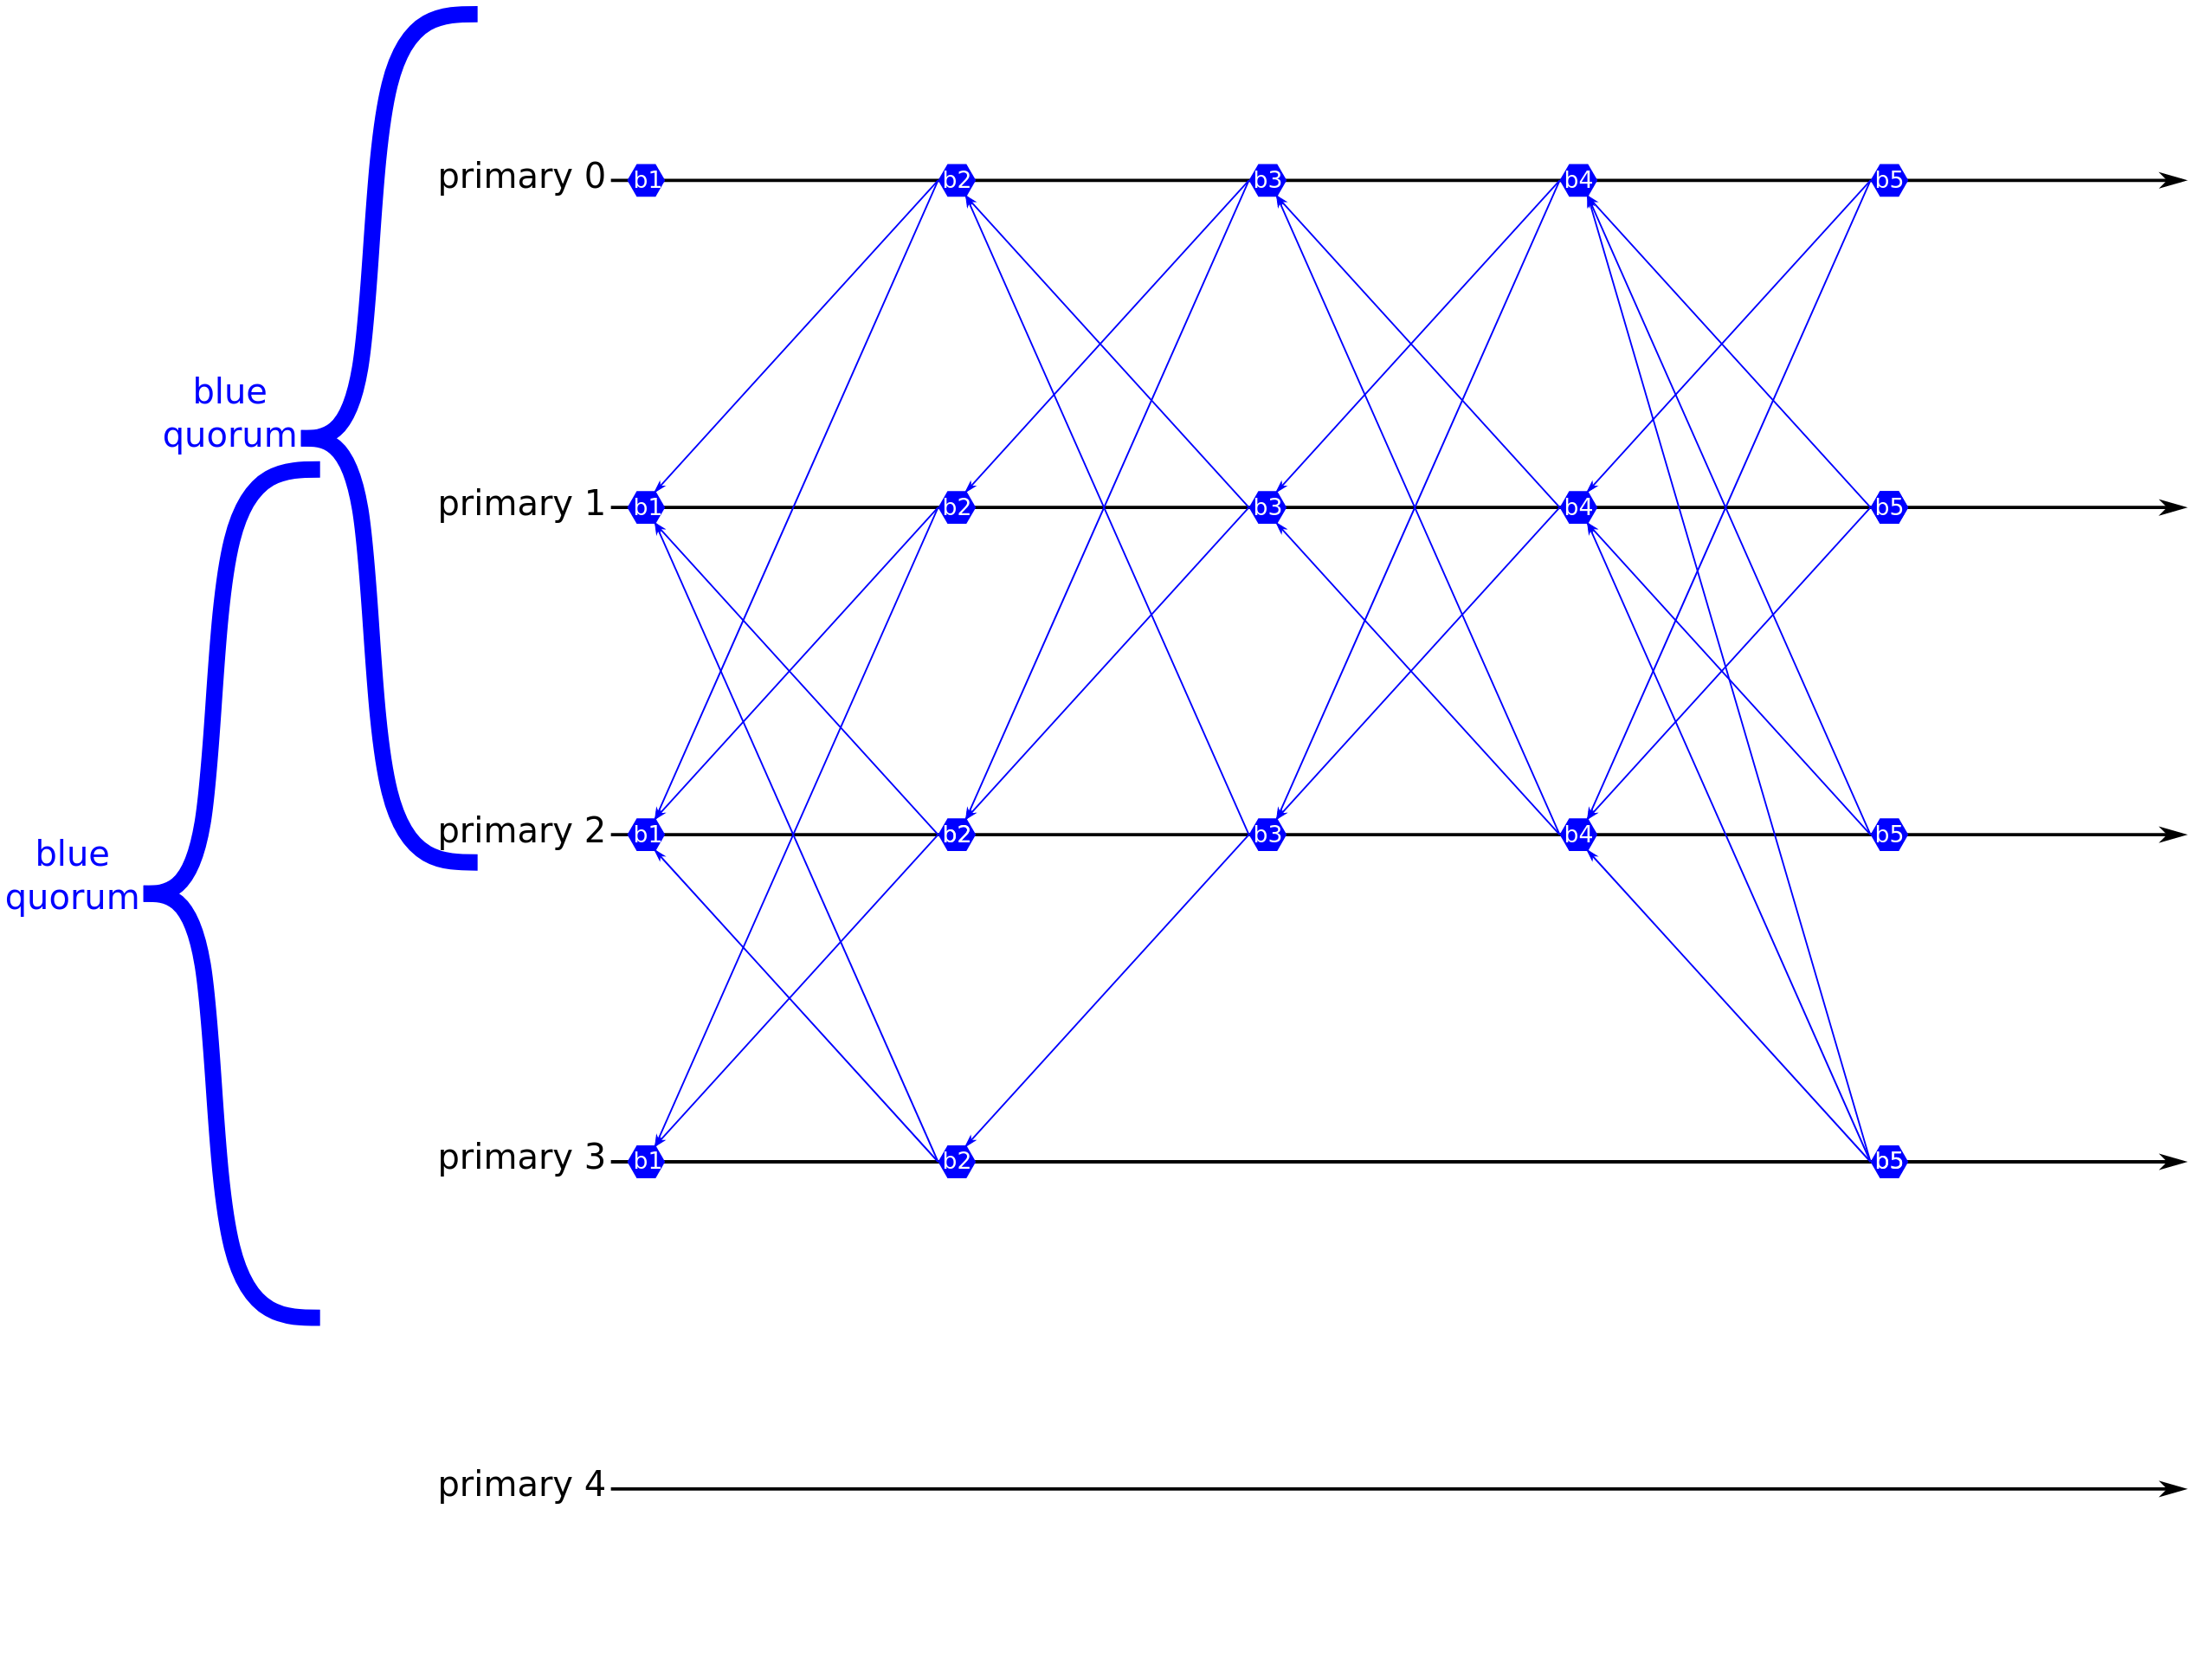
\includegraphics[width=.95\linewidth]{./blue_dag.png}
  \caption{A mem-\Dag (self-references omitted)}
  \label{fig:blue_dag}
\end{figure}


\begin{figure}[htb]
  \centering
  
  \begin{tikzpicture}
    \node[draw] (avl) {transaction data};

    \node[draw,right=1ex of avl] (dag) {``causal'' \Dag structure};
    \begin{pgfonlayer}{background}
    \node (x) [fill=lightgray,fit=(avl)(dag)] {};
  \end{pgfonlayer}
  \node[above=2ex of x,draw,double] {uniqueness of headers};
\end{tikzpicture}\protect\todo{where to put the signed quorums ?!}
  \caption%
  [Interdependence of availability and integrity]%
  {Illustration of 
    the interdependence of the availability and 
    integrity protocols}
  \label{fig:availability-n-integrity}
\end{figure}



Roughly, we have two complementary protocols running concurrently: 
 \begin{enumerate}
 \item the availability protocol; and
 \item the integrity protocol. 
 \end{enumerate}
 The availability protocol makes sure
 that transaction data is available 
 as long as necessary;\footnote{%
   There is some fine print concerning 
   the conditions under which this is actually the case. 
 }
 moreover,
 the availability protocol 
 is tasked with keeping available 
 the \emph{signed headers},
 \todo[inline]{explain \texttt{signed headers}}
 which the integrity protocol produces. 

 The integrity protocol makes sure that 
 each validator can only produce one block in each of its (local) rounds. 


 

\section{Architecture and communication patterns}
\label{sec:communication-patterns}
 We incorporate Narwhal's~\cite{NT} 
 scale out architecture%in our availability protocol 
 : %
 each validator has a unique \emph{primary} and % 
 a number of \emph{workers} % 
 (see \fig\ref{fig:validators})%
 . 
\begin{figure}[htb]
  \centering

validator:\(\left\{\begin{tikzpicture}[baseline={(p.south)},remember picture]
    \node[circle,draw,inner sep=1.5ex] (p) at (5.5,1.2) {p};
    \foreach \i in {1,...,10}{
      \coordinate (p_\i) at  (p.160+20*\i);
    }
    \foreach \i in {1,...,10}{
      \node[rectangle,fill=lightgray](w_\i) at (\i,0){\(w_{\i}\)};
      \draw[->] (w_\i.north) .. controls +(0,.2) .. (p_\i);
    }
    \begin{pgfonlayer}{background}
      \node[rounded corners,fill=blue!30!white,inner sep=2ex] (background) [fit=(w_1.south west)(w_10.south east)(p)] {};
    \end{pgfonlayer}
  \end{tikzpicture}\right.\)

\vspace{4ex}

\tikz[remember picture]{\node[rectangle,fill=gray,draw] (c) {client};}\hfill~\\

\vspace{4ex}

validator:\(\left\{\begin{tikzpicture}[baseline={(q.north)},remember picture,yscale=-1]
    \node[circle,draw,inner sep=1.5ex] (q) at (5.5,1.2) {q};
    \foreach \i in {1,...,10}{
      \coordinate (q_\i) at  (q.200-20*\i);
    }
    \foreach \i in {1,...,10}{
      \node[rectangle,fill=lightgray](v_\i) at (\i,0){\(v_{\i}\)};
      \draw[->] (v_\i.south) .. controls +(0,.2) .. (q_\i);
    }
    \begin{pgfonlayer}{background}
      \node[rounded corners,fill=blue!30!white,inner sep=2ex] (background) [fit=(v_1.north west)(v_10.north east)(q)] {};
    \end{pgfonlayer}
    % --------------------------------------------------------------------------------
    \begin{scope}[overlay,thick]
          \foreach \j in {1,...,10}
    \draw[<->] (v_\j) -- (w_\j);

    \draw[<->] (c.-15) .. controls +(2,0) and +(-1,-1) .. (v_3.north west);
    \draw[<->] (c.15) .. controls +(2,0) and +(-1,1).. (w_7.south west);
    \draw[<->] (p) -- (q);
    \end{scope}
  \end{tikzpicture}\right.\)
  \caption{The structure and communication patterns of validators}
  \label{fig:validators}
\end{figure}



\section{Preliminaries}
\label{sec:preliminaries}
\todo[inline]{%
  ``copy'' relevant parts of % 
  the heterogeneous paxos tech report%
}

Let us fix an arbitrary learner graph. 

\begin{definition}[Global Weak Quorum]
  \label{def:global-weak-quorum}
  A %
  \emph{global weak quorum} %
  is a set~\(X\) that is a weak quorum for each learner,  %
  i.e., \(X ∩ qₐ ≠ ∅\) %
  for every learner~\(a ∈ \Learner\), and %
  all \(qₐ ∈ \Q{a}\).
\end{definition}

\begin{definition}[Universal Quorum]
  \label{def:universal-quorum}
  A universal quorum is a set
  that contains a qourum for each learner. 
\end{definition}
\todo{%
“upward” closure for live quorums seems a “wrong” assumption
}


\section{Worker actions}
\label{sec:worker-actions}
Every validator has the same number of workers. 
Thus,
each worker can be assigned a unique \emph{mirror worker} 
on every other validator.
We shall adopt the convention of using the same subscript
for mirror workers of each other. % 
Thus,
in \fig\ref{fig:validators},
workers~\(w_2\) and~\(v_2\) are mirror workers of each other.
In the integrity protocol,
workers are only tasked with “bookkeeping” matters; 
in particular,
they keep track of (batches of) transactions,
their hashes,
and erasure coding shares;
they only pass on hashed data and 
block header information to their primaries.
The idea is to keep the network bandwidth usage of primaries 
as low as possible. 
For example,
primaries do not need to send messages back to their workers. 

\subsection{The pure availability protocol: worker actions}
\label{sec:base-protocol}
\todo[inline]{get rid of the broadcast of the availability certificates}
\todo[inline]{%
  maybe we need to ``announce'' headers, % 
  to avoid ``crossing'' of round numbers of learner%
}
\todo[inline]{%
  so, signed qourums are an ``output'' of the integrity protocol,
  and need to be made available (such that it is possible to create new headers). 
}

\todo[inline]{%
  worker hashes also should include an availability certificate %
  of the header creator's previous header %
}

\begin{description}
\item[Transaction collection (\tx{}←)] 
  \tnote{worker\\ ← client}
  Each worker keeps listening 
  for new transaction requests from clients.\footnote{%
    The bandwith and amount of storage for storing incoming transactions
    \emph{should} be big enough 
    to process all incoming transactions. 
    We share this assumption with Byzantine set consensus \cite{RedBelly}. 
    Transaction fees are one way to avoid flooding attacks,
    making the latter prohibitively expensive. 
    For example,
    we might assume a \fifo-buffer
    although it is more likely
    a priority queue,
    based on a combination of fees and
    quality of service considerations. 
  }
  Transactions should be buffered using reasonably fast memory. 
  \endnote{%
    This matter should be discussed
    in the context of \textsc{p2p}. 
  }

\item[Transaction distribution (\tx⇒)]
  \tnote{worker\\ ⇒ worker}
  Each worker “broadcasts” erasure coding shares of 
  every received transaction to mirror workers.
  In the simplest case\xspace% 
  ---the one we cover first---%
  this amounts to broadcasting the transaction.\footnote{ 
  However, 
  if we perform proper erasure coding,  
  it is not broadcasting in the strict sense:
  each mirror worker receives a different message. 
  We first cover the case of trivial erasure coding
  ‼[covering the case of proper erasure codining in ‽].
  }
  In general,
  transaction distribution can be divided into two steps.
  \todo[inline]{
    we might require a 
    \emph{position number} for
    transactions of the current batch, 
    and a sequence number (of the block to be produced)
  }
  \begin{description}
  \item[Erasure coding via copying (\es)]
    \tnote{[worker]}
    We first cover the case of trivial erasure coding, 
    in line with the description of the homogeneous case~\cite{NT}. %
    Thus, erasure coding shares of a transactions are simply copies. 
    We visually distinguish between “copies” of transactions
    from the “original” transaction supplied by the client,  
    using the symbols \tx\ and \es, respectively. 
%%%%%%%%%%%%%%%%%%%%%%%%%%%%%%%%%%%%%%%%%%%%%%%%%%%%%%%%%%%%%%%%%%%%%%%%%%%%%%%%%%%%%%%%%
    \todo[inline]{put fwd ref / future work }
%%%%%%%%%%%%%%%%%%%%%%%%%%%%%%%%%%%%%%%%%%%%%%%%%%%%%%%%%%%%%%%%%%%%%%%%%%%%%%%%%%%%%%%%%    
  \item[Copy distribution (\es⇒)] 
    \tnote{worker\\ ⇒ worker }
    Each share of the erasure code,
    \ie a copy of the transaction, 
    is sent to every mirror worker.%
    \endnote{
      elaborate on the distribution scheme,
      and how the destination of each earasure share is determined
      (for the general erasure coding).
    }%
    \xspace
    We tag each transaction with a \emph{sequence number},
    consisting of the validator round and 
    the position in the list of transactions for 
    the next block (header) in which the transaction will be included. 
    % so that it becomes clear in which order the 
    % transactions of the next block (header) will be listed. 
  \end{description}
  Note that copies of transactions are \emph{not} signed by the worker. 
  Signatures are deferred to until after the last transaction  
  of a validator round, 
  when the worker will sign the hash of the list of all broadcast transactions,
  called a \emph{worker hash}. 
  
\item[Worker hash compilation (\wh)]
  \tnote{(worker)}
  Towards the end of a “validator round”,\endnote{%
    Is there any such thing as “validator round”?\\
    - sequence number\\
    - validator height\\
    - ... 
  }%
  \xspace
  each worker produces its worker hash for the broadcast batch of transactions. 
  In detail,
  a worker hash consists of 
  \begin{itemize}
  \item the hash of the broadcast list of transactions,
  \item the number of transactions, and
  \item the round number,  
  \end{itemize}
  signed by the worker. 
  \endnote{\color{red}
    For general erasure coding:
    \em Does this need to includes for each receiving worker,
    the (hashes of the) erasure coding shares that 
    they should have available. ?
  }
\item[Worker hash broadcast (\wh⇒)] 
  \tnote{worker\\ ⇒ worker }  
  A worker broadcasts its most recent worker hash
  to mirror workers.
\item[Worker hash provision (\wh↑)]
  \tnote{worker\\ → primary}
  The most recent worker hash is sent to the primary 
  for inclusion into the next header. 
  \todo{
    How much “additional” information do we have 
    to include into the header
    such that signing a header certificate becomes meaningful?
  }
  
\item[Worker hash reception and checking ({\wh[]←})] 
  \tnote{worker\\ ← worker}  
  At any time, 
  a worker can receive a worker hash 
  from a mirror worker. 
  As a first reaction, 
  it checks whether enough 
  transactions have been received by the worker and, 
  if so, 
  whether the hash of the list of transaction matches the worker hash. 

\item[Worker hash forward ({\wh[]⇑})]
  \tnote{worker\\ → primary}  
  If a worker has successfully checked 
  the availability of the transactions of a received worker hash, %
  it “forwards” the worker hash to its primary.\footnote{%
    Validators will use this information 
    to send availability commitments to block headers of other primaries.
  }
\end{description}



\begin{figure}[htb]
  \centering
  \tikzstyle{every node}+=[outer sep=0pt,inner sep=1pt]
  \newcommand{\primaryDistance}{15ex}
  \newcommand{\workerPrimaryDistance}{1ex}
  \newcommand{\workerDistance}{3ex}
  \scalebox{.9}{%
  \footnotesize%
  \begin{tikzpicture}[scale=1.2]
    %%%%%%%%%%%%%%%%%%%%%%%%%%%%%%%%%%%%%%%%%%%%%%%%%%%%%%%%%%%%%%%%%%%%%%%%%%%%%%%% 
    % The message passing diagram of the availability protocol at genesis
    %%%%%%%%%%%%%%%%%%%%%%%%%%%%%%%%%%%%%%%%%%%%%%%%%%%%%%%%%%%%%%%%%%%%%%%%%%%%%%%%
    % first the time lines for primaries and their workers
    \coordinate (primaryAnchor) at (0,0);
    \foreach \p in {1,...,5} {
      \node[below=\primaryDistance of primaryAnchor,anchor=east] (p\p) 
      at (primaryAnchor) {\ensuremath{\text{primary}_\p}};
      \draw[->] (p\p) -- ++(10.4,0);
      \coordinate (workerAnchor) at ([yshift=-\workerPrimaryDistance]p\p.east);
      \foreach \j in {1,...,2} {
        \node[below=\workerDistance of primaryAnchor,anchor=east] (w\p_\j) 
        at (workerAnchor) {\ensuremath{\text{worker}_{\p,\j}}};
        \draw[->] (w\p_\j) -- ++(10.4,0) ;
        \coordinate (workerAnchor) at (w\p_\j.east);
      }
      \coordinate (primaryAnchor) at (p\p.east);
    }
    %%%%%%%%%%%%%%%%%%%%%%%%%%%%%%%%%%%%%%%%%%%%%%%%%%%%%%%%%%%%%%%%%%%%%%%%%%%%%%%% 
    % a first transaction tx1
    \node (tx1) at ([xshift=3.5ex]w1_1.east) {\tx₁};
    \draw[->,double,dotted,shorten >=-2ex] (tx1.200) ++ (200:1em) -- (tx1);
    \foreach \p in {2,...,5} {
      \node (es\p_1) at ([xshift=6ex-\p ex]tx1|-w\p_1) {\es₁};
      \draw[->] (tx1) -- (es\p_1) ;
    }
    % a bunch of transactions tx2-5 that will make it into WHs actually
    \node (tx2) at ([xshift=3*3.5ex]w3_2.east) {\tx₂};
    \draw[->,double,dotted,shorten >=-2ex] (tx2.200) ++ (200:1em) -- (tx2);
    \foreach \p in {1,2,4,5} {
      \node (es\p_2) at ([xshift=6ex-\p ex]tx2|-w\p_2) {\es₂};
      \draw[->] (tx2) -- (es\p_2) ;
    }
    \node (tx3) at ([xshift=5*3.5ex]w3_2.east) {\tx₃};
    \draw[->,double,dotted,shorten >=-2ex] (tx3.200) ++ (200:1em) -- (tx3);
    \foreach \p in {1,2,4,5} {
      \node (es\p_3) at ([xshift=6ex-\p ex]tx3|-w\p_2) {\es₃};
      \draw[->] (tx3) -- (es\p_3) ;
    }
    \node (tx4) at ([xshift=7*3.5ex]w3_1.east) {\tx₄};
    \draw[->,double,dotted,shorten >=-2ex] (tx4.200) ++ (200:1em) -- (tx4);
    \foreach \p in {1,2,4,5} {
      \node (es\p_4) at ([xshift=6ex-\p ex]tx4|-w\p_1) {\es₄};
      \draw[->] (tx4) -- (es\p_4) ;
    }
    \node (tx5) at ([xshift=9*3.5ex]w3_1.east) {\tx₅};
    \draw[->,double,dotted,shorten >=-2ex] (tx5.200) ++ (200:1em) -- (tx5);
    \foreach \p in {1,2,4,5} {
      \node (es\p_5) at ([xshift=6ex-\p ex]tx5|-w\p_1) {\es₅};
      \draw[->] (tx5) -- (es\p_5) ;
    }
    % collection of txs into worker hashes wh1 and wh2
    \node[right=.1ex of tx5] (wh1) {\wh₁};
    \draw[dotted,bend right=2.5ex] (wh1.center) to (tx5.center);
    \draw[dotted,bend right=5ex] (wh1.center) to (tx4.center);
    \node[right=3.5ex of wh1|-tx3] (wh2) {\wh₂};
    \draw[dotted,bend left=2.5ex] (wh2.center) to (tx3.center);
    \draw[dotted,bend left=5ex] (wh2.center) to (tx2.center);
    %%%%%%%%%%%%%%%%%%%%%%%%%%%%%%%%%%%%%%%%%%%%%%%%%%%%%%%%%%%%%%%%%%%%%%%%%%%%%%%%
    % "upload" of worker hashes wh1 and wh2 to the primary, wh1' and wh2'
    \node (wh1') at ([xshift=-2ex]wh2|-p3) {\wh₁};
    \draw[->] (wh1) -- (wh1');
    \node[right=0ex of wh1'] (wh2') {\wh₂};
    \draw[->] (wh2) -- (wh2');
    % the following should be much later, but ... (single harmless hack)
    \node[right=1ex of wh2',fill=white] (hd3) {\hd};
    \foreach \k in {1,2}
    \draw[dotted,bend right=9ex-3*\k ex] (hd3) to (wh\k'.center);
    %%%%%%%%%%%%%%%%%%%%%%%%%%%%%%%%%%%%%%%%%%%%%%%%%%%%%%%%%%%%%%%%%%%%%%%%%%%%%%%%
    % dissemination of worker hashes wh1 and wh2
    \foreach \p in {1,2,4,5} {
      \node (wh1_\p_1) at ([xshift=3ex-\p ex]wh1'|-w\p_1) {\wh[]₁};
      \draw[->] (wh1) -- (wh1_\p_1) ;
    }
    \foreach \p in {1,2,4,5} {
      \node (wh2_\p_2) at ([xshift=6ex-\p ex]wh2'|-w\p_2) {\wh[]₂};
      \draw[->] (wh2) -- (wh2_\p_2) ;
    }
    %%%%%%%%%%%%%%%%%%%%%%%%%%%%%%%%%%%%%%%%%%%%%%%%%%%%%%%%%%%%%%%%%%%%%%%%%%%%%%%%
    % worker hash upload at receiving validators
    \foreach \whx in {1,2} { % for each of the two worker hashes
      \foreach \p in {1,2,4,5} { % for each "other" validator
        \node (wh\whx_\p_\whx') at ([xshift=4ex-\whx ex]wh\whx_\p_\whx|-p\p) {\wh[]\ensuremath{{}_\whx}};
        \draw[->] (wh\whx_\p_\whx) -- (wh\whx_\p_\whx');
        % and header creation (after second block)
        % ... and sending availability votes
        \ifthenelse{\equal{\whx}{2}}%
        {\node[right=2ex of wh\whx_\p_\whx',fill=white,draw=none] (hd\p) {\hd}; 
          \foreach \k in {1,2}
          \draw[dotted,bend right=9ex-3*\k ex] (hd\p) to (wh\k_\p_\k'.center);
        }%
        {}%
      }
    }
    %%%%%%%%%%%%%%%%%%%%%%%%%%%%%%%%%%%%%%%%%%%%%%%%%%%%%%%%%%%%%%%%%%%%%%%%%%%%%%%%
    % collect "foreign" whs into availability votes for a block
    \coordinate (ac) at ([xshift=2ex,yshift=2ex]hd1|-p3);
    \foreach \p in {1,2,4} { % for each "other" validator
      \node[fill=white] (av\p) at (ac){\hd\makebox[0pt][l]{\ensuremath{{}_{\sim\p}}}};
      \coordinate (ac) at ([xshift=-1ex,yshift=-1ex]ac);
    }
    \foreach \p in {1,2,4} { % for each "other" validator
      \draw[->] (hd\p) -- (av\p.east);
    }
    \node[fill=white] (av3) at (ac){\hd\makebox[0pt][l]{\ensuremath{{}_{\sim3}}}};
    \draw[->] (hd3) -- (av3);
    \begin{pgfonlayer}{background}
      \node[fit={(av3)(av1)([xshift=2ex]av1.north east)},fill=lightgray] (ac3) {};
    \end{pgfonlayer}
    % broadcast the availability certificate
    \foreach \p in {1,...,5} { % for each "other" validator
      \node (ac\p') at ([xshift=17ex-\p ex]ac|-p\p) {\ac\ensuremath{{}_\p}};
      \draw[->] ([yshift=2.5ex-\p ex]ac3.east) -- (ac\p'); 
    }
  \end{tikzpicture}%
  }
  \caption{The availability protocol in the genesis round}
  \label{fig:availability-protocol}
\end{figure}
%\end{comment}
\section{Primary actions}


\subsection{Availability at genesis}
The pure availability protocol: genesis actions

\begin{description}
\item[Genesis header compilation ({\hd[]})] 
  \tnote{[primary]}
  If a primary has obtained a complete set of 
  worker hashes for the genesis round
  from its workers, 
  it can compile a block header. 
  The process of header compilation 
  does not distinguish between worker hashes of its local workers
  and those with transactions that were received at other validators. 
  At genesis,
  the header consists of the creator's identity 
  and the list of worker hashes.
  
\item[Availability voting/commitment (\hdₚ→)]
  \tnote{primary\\ → primary}
  A genesis header of a primary is acceptable 
  if all its worker hashes have been forwarded
  by the local workers
  (which are trusted to have checked these worker hashes).
  The latter implies that the relevant erasure coding shares
  are kept available. 
  An availability commitment is made
  by signing the header 
  and sending the signed header to the creator
  (for the purpose of aggregation into availability certificates). 

\item[Commitment aggregation (\hdₚ←)]
  \tnote{[primary]}
  The signatures of received availability commitments 
  are aggregated into certificates of availability 
  for a header. 

\item[Certificate broadcast (\ac⇒)]
  \tnote{primary\\ ⇒ primary}
  Once a primary receives commitments
  from a global weak quorum for its genesis header,
  it broadcasts the certificate of availability.  

\item[optional header distribution] 
  ~\todo[inline]{%
    Right now,
    there seems no reason to add this ``safe guard'';
    it might be confusing.
  }
  One might expect that header creators send their headers around.
  However,
  there is no need for this.%
  \endnote{... at least in theory, we'll keep it slick for the moment} 
  
  % has uploaded a worker hash 
  % for the genesis round, 
  % optionally, 
  % the primary \emph{can} distribute 
  % the genesis header:
  % ‼{\color{red} why do we do this then at all?}
  % \begin{itemize}
  % \item the primary~\(p\)
  % \item worker hashes \(\wh_1 \cdots \wh_n\), 
  %   produces by the local workers at \(p\)'s validator. 
  % \end{itemize}
  % In theory,
  % this step is not necessary,
  % since each other primary will eventually receive
  % the  worker hashes \(\wh_1 \cdots \wh_n\),  
  % forwarded from it's workers. 
  
  % Note,
  % the creating primary of the header does not sign it;
  % the signature is “delayed” until 
  % enough primaries have commited to storing 
  % the underlying data,
  % as described by the next action.

  % ‼[a “sequence number” with the set of “target” learners should suffice,
  % to trigger such an header request]
\end{description}

A (partial) execution of the availability protocol at genesis is
illustrated in \fig\ref{fig:availability-protocol}.

\FloatBarrier

\subsection{Integrity: the general case at once}
First off,
the integrity-protocol
re-uses the sending of signed headers~\(\hdₚ\) to the creator 
(from the availability-protocol), 
as a commitment of the signer to 
one unique header for the  validator (and round),  
namely the first one signed and sent. 
Thus, 
correct validators will not sign and send any other header 
for the respective  creator of the header (for the same round). 


\begin{description}
\item[Integrity signing \(\hdₚ\)]
  \tnote{primary ⇒ primary}
  Signing and sending the header to the creator implies that 
  (a correct) primary will not sign any other header
  of the same creator with the same round number. 

\item[Block aggregation (\bk)]
  \tnote{[primary]}
  Using 
  the same signature aggregation mechanism that
  is used for availability certificates, 
  validators will aggregate additional signatures 
  (besides the availability signature) for their block headers,
  producing learner-specific \emph{blocks}, 
  which, by definition, 
  are headers signed by a learner-specific quorum. 

\item[Block broadcast \(\bk\)] 
  \tnote{primary ⇒ primary}
  The aggregated signatures of a block header form 
  a \emph{learner-specific block}. 
  The signature aggreator will broadcast 
  to all primaries that belong to some quorum of the respective learner. 
  (Later,
  these will be used as references to 
  previous blocks in the learner-specific \Dag[s]
  see \ref{???}) %FIXME reference.
\end{description}

There is no conceptual difference between 
the integrity protocol at genesis,
comparted to the typical case. 
The only difference is that 
headers in the general case 
will carry additional information. 
Thus,
we can finish the description of the protocol, 
by filling in the additional data and steps in the typical phase
of the availability-protocol 
(see also \fig\ref{fig:data-structures},
for the difference between headers at genesis and the typical phase). 

\begin{figure}[htb]
  \centering
  \tikzstyle{every node}+=[outer sep=0pt,inner sep=1pt]
  \newcommand{\primaryDistance}{15ex}
  \newcommand{\workerPrimaryDistance}{1ex}
  \newcommand{\workerDistance}{3ex}
  \scalebox{.8}{%
    \footnotesize%
    \begin{tikzpicture}[scale=1,thick]
      %%%%%%%%%%%%%%%%%%%%%%%%%%%%%%%%%%%%%%%%%%%%%%%%%%%%%%%%%%%%%%%%%%%%%%%%%%%%%%%% 
      % The message passing diagram of the integrity protocol
      %%%%%%%%%%%%%%%%%%%%%%%%%%%%%%%%%%%%%%%%%%%%%%%%%%%%%%%%%%%%%%%%%%%%%%%%%%% 
      \coordinate (primaryAnchor) at (0,0);
      \foreach \p in {1,...,7} {
        \node[below=\primaryDistance of primaryAnchor,anchor=east] (p\p) 
        at (primaryAnchor) {\ensuremath{\text{primary}_\p}};
        \draw[->] (p\p) -- ++(15,0);
        \coordinate (primaryAnchor) at (p\p.east);
      }
      \begin{pgfonlayer}{background}
        \foreach \p in {1,...,4}{
          \node[pattern=crosshatch, pattern color=green!80!black,fit={(p\p)},inner sep=1.5ex] {};
          \node[fill=white, fit={(p\p)}] {};
        }
        \foreach \p in {1,3,5,7}{
          \fill[pattern=horizontal lines, pattern color=blue]
          (p\p.north east) -- (p\p.south west) -- (p\p.south east) -- cycle;
        }
        \foreach \p in {3,...,7}{
          \fill[pattern=vertical lines, pattern color=blue]
          (p\p.north east) -- (p\p.south west) -- (p\p.north west) -- cycle;
        }
      \end{pgfonlayer}

      \node[inner sep = 4ex] (theOrigin) at ([xshift=-3ex]p3.10) {};
      \foreach \p in {1,...,7} { % for each "other" validator
        \coordinate (ac\p') at ([xshift=17ex-\p ex]theOrigin|-p\p) ;
    }
    \node (ac3') at ([xshift=17ex-3 ex]theOrigin|-p3) {\ac\ensuremath{{}_3}};
    \draw[->] (theOrigin) -- ([xshift=4ex,yshift=4ex]ac3'); 
    \coordinate[right=14ex of ac3'] (sigAgg);
    \foreach \p in {1,2,4} { % for each "other" validator
      \node[fill=white] (av\p) at (sigAgg){\hd\makebox[0pt][l]{\ensuremath{{}_{\sim\p}}}};
      \coordinate (sigAgg) at ([xshift=-1ex,yshift=-1ex]sigAgg);
    }
    \foreach \p/\y in {1/2,2/1,4/-14} {
      \node[left=\y ex of ac\p',fill=white] (hd\p') {\hd};
      \draw[->] (hd\p') -- (av\p);
    }
    \begin{pgfonlayer}{background}
      
      \node[fit={(av4)([xshift=2ex]av1.north east)([xshift=-2ex]ac3'.west)},pattern=crosshatch,pattern color=green!80!black,draw] (bkGreen) {};
    \end{pgfonlayer}
    \foreach \p in {1,...,4} { % for each "green" validator
      \node[right=25 ex of ac\p'] (bkGreen\p') {\bk};
      \draw[->] (bkGreen) -- (bkGreen\p'); 
    }
    \foreach \p in {5,...,7} {
      \node[right=35 ex of ac\p',fill=white] (hd\p') {\hd};
      \draw[->] (hd\p') -- (ac\p');
    }
    \coordinate[right=15 ex of bkGreen3'] (sigAgg);
    \foreach \p in {7,...,5} { % for each "other" validator
      \node[fill=white] (av\p) at (sigAgg){\hd\makebox[0pt][l]{\ensuremath{{}_{\sim\p}}}};
      \draw[->] (hd\p') -- ([xshift=1ex,yshift=-.5ex]av\p.south east);
      \coordinate (sigAgg) at ([xshift=-1ex,yshift=-1ex]sigAgg);
    }
      \begin{pgfonlayer}{background}
        
        \node[fit={(bkGreen3')([xshift=2ex]av7.north east)(av5)},pattern=vertical lines,pattern color=blue,draw] (bkBlue) {};
      \end{pgfonlayer}
    \foreach \p in {7,...,3,1} { % for each validator in some "blue" quorum, 
      \node[right=65 ex of ac\p'] (bkBlue\p') {\bk[blue]\ensuremath{{}_3}};
      \draw[->] (bkBlue.east) -- (bkBlue\p'); 
    }
    \coordinate (top) at (bkBlue3'.east|-p1); 
    \coordinate (bottom) at (bkBlue3'.east|-p7); 
    \draw[double,very thick,dotted] ([xshift=1ex,yshift=1ex]top) -- ([xshift=1ex,yshift=-1ex]bottom);
    \coordinate (sigAgg) at ([xshift=20ex]bkBlue5');
    \foreach \p in {7,...,4} { % for each "other" blue validator, not 3
      \node[fill=white] (bk\p) at (sigAgg){\bk[blue]\makebox[0pt][l]{\ensuremath{{}_\p}}};
      %\draw[->] (bk\p') -- ([xshift=1ex,yshift=-.5ex]av\p.south east);
      \coordinate (sigAgg) at ([xshift=-1ex,yshift=-1ex]sigAgg);
      \draw[->] (sigAgg|-p\p) -- (bk\p.south east);
    }    
    \begin{pgfonlayer}{background}
      \node[fit={(bkBlue5')([xshift=2ex]bk7.north east)(bk4.south west)},fill=lightgray] (BlueBlocks) {};
    \end{pgfonlayer}
    \foreach \p in {3,5,6,7} {% for some blue learners
      \node[draw=blue] (qs\p) at ([xshift=5ex]BlueBlocks.east|-p\p) {\qs[5]};
      \draw (BlueBlocks.east) -- (qs\p);
    }
  \end{tikzpicture}%
    \todo{for cooler patternage
      \url{https://tex.stackexchange.com/questions/597172/tikz-set-the-line-width-of-the-pattern}
    }
  }
  \caption[Integrity protocol]{%
    The integrity protocol 
    (concluding each round that's was “opened” in the availability-protocol)%
  }
  % 
  \label{fig:integrity-protocol}
\end{figure}
\todo[inline]{%
  blue blocks go to all validators in 
  %\begin{enumerate}
  % \item
  ① the signing quorum
  % \item
  ② all validators that are in some blue quorum 
  %\end{enumerate}
}

\subsection{Availability: the typical case}

\begin{description}
\item[Generating and broadcasting signed quorums]
  \tnote{primary \\⇒ primary}
  Once a validator has collected 
  enough new  blocks (for a learner), 
  it signs a learner-specific quorum of such blocks;
  the result is called a \emph{signed quorum},  
  for short. 
  All these blocks have to be from the same round. {\color{red} important ‼}

  Under certain conditions,
  in particular if there is exceptional delay for a specific learner,
  one can forgoe announcing a proper signed quorum
  and instead signs a \emph{dummy quorum} for a specific learner,
  \ie a signature over the ID of the learner in question and the current round number.  

\item[General header compilation]
  The biggest additional work and data
  concerns the compilation of headers.
  In the typical phase, 
  a header carries two additional data items, namely
  \begin{itemize}
  \item 
    the availability certificate of the previous header 
    of the header's creator/initiator
  \item 
    hashes of the signed (dummy) quorums sent by the same validator
  \end{itemize}

\item[General header checking]
  As signed quorums also serve as certificates of availability,
  checking a signed quorum amounts to checking the signed certificates.\endnote{%
    Somehow it seems overkill to have (hases of) signed quorums in the headers.   }
  In a similar way,
  the certificate of availability amounts to a checking of signatures.
\end{description}

\todo[inline]{describe in detail how 

  the checking of the availability of the headers takes place}

\subsection{Summary}
The availability protocol in a non-genesis round 
only differs in having
\begin{enumerate}
\item the additional requirement 
that each block header also includes 
the certificate of availability 
for the previous header of the same validator and 
\item 
the sending and checking of signed quorums
(each of which implements the reference to 
blocks from the previous round—in a learner-specific \Dag).
\end{enumerate}

As a consequence,
casting an availability vote / sending a commitment message 
\todo{discuss terminnolgy}
becomes a recursive commitment
to storing all blocks until genesis 
(or the last block that some of learners might still want availabl). 

\section{Data structures}

\begin{figure}[htb]
  \centering
% \subfloat[\color{violet} \bf Missing]{
%   \begin{minipage}{.3\linewidth}
%       \begin{itemize}
%   \item Integrity Vote (cf. Availability Vote → Storing promise ?)
%   \item ~ 
%   \end{itemize}
%   \end{minipage}
% }

  \subfloat[Transaction received by worker~\(w\)]{
    \tx:
    \begin{tikzpicture}[baseline={([yshift=-.5ex]b.center)}]
      \node[ellipse,fill=black] (b){
        \textcolor{white}{\bf\footnotesize\begin{tabular}[c]{c}
                                            trasaction\\
          data
        \end{tabular}}
    };
    \node[anchor=west] (w) at (b.south east) {\small\({}\to w\)};
    \end{tikzpicture}
  }
  \qquad
  \subfloat[Transaction copy (trivial erasure share)]{
    \es: \tx
    % \begin{tikzpicture}[baseline={([yshift=-.5ex]b.center)}]
    %   \phantom{
    %   \node[ellipse,fill=black] (b){
    %     \textcolor{white}{\bf\footnotesize\begin{tabular}[c]{c}
    %       blob\\
    %       of\\
    %       data
    %     \end{tabular}}
    %   };}
    % % https://texample.net/tikz/examples/torn-paper/ 
    % % ‼ make cute torn edges
    % \clip[fill] ([xshift=-1em]b.north east)
    % -- ([yshift=1em]b.south west) 
    % -- ([xshift=1em]b.south west)
    % -- ([yshift=-1em]b.north east) -- cycle;
    % \node[ellipse,fill=black] (b){
    %     \textcolor{white}{\bf\footnotesize\begin{tabular}[c]{c}
    %       blob\\
    %       of\\
    %       data
    %     \end{tabular}}
    %   };
    % \end{tikzpicture}
}
  % \qquad
  % \subfloat[Worker \(y\) is commiting to the hash of~\(x\)]{
  %   \(y♯x\): \([\#(x)]_{\sim y}\)
  % }%‼

\subfloat[Batch hash of worker~\(w\)]{
  \#(\(\overrightarrow\tx\)):
  \#
    \(\left(\begin{tikzpicture}[baseline={(batch.center)}]
      \node[anchor=west] (batch) {
        \(\colorbox{lightgray}{\(\begin{array}[c]{c}
          {\tx}\\%_{\to w}
          {\tx}\\%_{\to w}
          {\tx}\\%_{\to w}
          {\tx}\\%_{\to w}
          {\tx}\\%_{\to w}
          {\tx}%_{\to w}
        \end{array}\)}\)
    };
      \end{tikzpicture}\right)\)
  }
  \subfloat[%
  Worker hash (issued by~\(w\)), 
  including the round number \(\rnd\),
  and the number of transactions~\(\|\protect\overrightarrow \tx\|\);
  it is signed by~\(w\)]{
    \wh:
    \begin{tabular}[t]{@{}l@{}}
      \begin{tikzpicture}[baseline={([yshift=-.5ex]wh.center)}]
        \node (wh){\(\left[ \#(\overrightarrow \tx), \rnd,  \|\overrightarrow \tx\| \right]_{w}\)}; 
      \end{tikzpicture}
      %\footnotesize
    % {\color{violet} + info for correctness checking} \\
    % (\eg number of \tx[s], or list of \#s)\\
    %   \emph{Tahoe – The Least-Authority Filesystem}
    \end{tabular}
  }

  \subfloat[Genesis Header]{
    \(\hd[]\):\(
\tikz[baseline={(x.base)}]{\node (x){
\(\left(p,\overrightarrow\wh\right)\)
};}\)
  }
\qquad
  \subfloat[Genesis certificate of availability]{
    \(\ac\): 
    \(\Bigl[\hd[]\Bigr]_{\overrightarrow q}\)
  }

  \subfloat[Block]{
\bk:
    \begin{math}
      \left[\hd\right]_{\color{green!60!black}{\sim p_1 \dots \sim p_m} [ \color{green!60!black}\sim p_{m+1} \cdots \sim p_{k}]}
    \end{math}
  }
  \qquad
  \subfloat[Signed quorum]{
    \(\qs_p\):
    \begin{math}
      \begin{array}[c]{@{\rhd}l}
        [\bk_1 \cdots \bk_\ell]_{\sim p}
      \end{array}
    \end{math}
  }

  \subfloat[Header]{
    \(\hd\):\(
\tikz[baseline={(x.base)}]{\node (x){
\(\left(p,\overrightarrow\wh,\ac, \overrightarrow {\#(\qsₚ)}\right)\)
};}\)
  }


  \caption{Overview of data structures}
  \label{fig:data-structures}

\end{figure}
\FloatBarrier






\bibliographystyle{alpha}
\bibliography{HN.bib}


\appendix
\printendnotes
\end{document}


%%% Local Variables:
%%% mode: latex
%%% TeX-master: t
%%% TeX-engine: luatex
%%% TeX-command-extra-options: "-shell-escape"
%%% End:
